\documentclass[a4paper,DIV=12,english]{scrartcl}
\usepackage[utf8]{inputenc}
\usepackage{fancyhdr}
\usepackage{bookmark}
\usepackage{graphicx}
\usepackage{hyperref}
\usepackage{xurl}
\usepackage[sorting=none, style=numeric-comp]{biblatex}
\addbibresource{ref.bib}
\usepackage{csquotes}
\usepackage[dvipsnames]{xcolor}
\usepackage[num]{isodate}
\usepackage{amsthm}
\usepackage{amssymb}
\usepackage{bbm}
\usepackage{amsmath}
\usepackage{tikz}
%\usepackage{pgfplots}
    %\usepgfplotslibrary{fillbetween}
\usepackage{svg}
\usepackage{braket}
\usepackage{caption}
\usepackage{subcaption}
\usepackage{placeins}
%\setlength\parindent{0pt}
\usepackage{wrapfig}
\usepackage{float}


% Fakesection
\newcommand{\fakesection}[1]{%
    \par\refstepcounter{section}                                        % Increase section counter
    \sectionmark{#1}                                                    % Add section mark (header)
    \addcontentsline{toc}{section}{\protect\numberline{\thesection}#1}  % Add section to ToC
    % Add more content here, if needed.
} 

\renewcommand{\footrulewidth}{0.5pt}
\pagestyle{fancy}
\fancyhf{}
\fancyhead[L]{\leftmark}
\fancyhead[R]{}

\fancyfoot[C]{Computational Physics: Eigenvalue Problems 1}
\fancyfoot[R]{\thepage}

\title{Computational Physics: Eigenvalue Problems 1}
\author{Stockholm University, Spring Term 2024 \\Max Maschke}
\date{Apr 11 2024}


\begin{document}
\maketitle


\tableofcontents
\newpage


\newpage
\section{Introduction}
The aim of this project is to implement a numerical solver for the 1D-Schrödinger equation and test it for the harmonic oscillator. It is part of the coursework for the computational physics class held at Stockholm University in 2024.

\section{Method}
\subsection{Discretising the 1D Schrödinger Equation}
The time independent Schrödinger equation (SEQ) is famously an eigenvalue problem: 
\begin{equation}\label{SEQ}
    \mathcal{H}\ket{\psi} = E\ket{\psi}
\end{equation}
For a single particle and moving to real-space representation, using the wave function $\psi(x) = \braket{x|\psi}$, it assumes the form 
\begin{equation}
    \left(-\frac{\hbar^2}{2m}\partial_x^2 + V(x)\right)\psi(x) = E\psi(x)
\end{equation}
where $V(x)$ is the real-space representation of the potential operator $\mathcal{V}$, which is a diagonal operator in this basis. $\mathcal{H}$ itself is, however, not diagonal, which is why, considering the difficulty of obtaining analytical solutions to the SEQ, one might be interested in numerical approaches to the eigenproblem posed.

The first necessary step is to translate the infinite dimensional problem stated above into a finite basis. Naturally, this involves some sort of approximation. Intuitively, one possible approach is to go from the infinite dimensional eigenbasis of the position operator $\mathcal{X}$
\begin{equation}\
    \mathcal{X}\ket{x} = x\ket{x},\quad \braket{x'|x}=\delta(x'-x), \quad x \in \mathbb{R}
\end{equation}
to a discretised set of positions $x_i$ with an associated discrete position operator $X$
\begin{equation}
    X \ket{x_i} = x_i \ket{x_i}, \quad \braket{x_j|x_i} = \delta_{ij}, \quad i \in \mathbb{N}.
\end{equation}
If we additionally impose a maximum and minimum value of $x_i$ (N.B.\ this implies assuming $\psi(x)=0$ outside for the purposes of finding solutions to the SEQ) and require neighbouring positions to have constant spacing $h$, the set of allowed positions assumes a finite number $n$:
\begin{equation}
    x_i = x_\text{min} + i \cdot h, \quad i = 0, \dots, n -1
\end{equation}
It will be convenient to set $x_\text{min} = -x_\text{max}$ henceforth. For a given $n$, that yields
\begin{equation}
     h = 2x_\text{max}/(n-1).
\end{equation}
What we have achieved by moving to this finite basis is that, if we can map $\mathcal{H}$ to its finite representation $H\in\mathbb{C}^n$,~\eqref{SEQ} can be represented as a matrix equation, which allows us to unleash the whole toolbox of numerical linear algebra onto it. Moreover, any real function $\mathcal{F}$ on $[-x_\text{max}, x_\text{max}]$ can be represented by a vector $f\in\mathbb{R}^n$ by the identification
\begin{equation}
    f = \sum_i f(x_i) e_i.
\end{equation}
Naturally, this also applies to the wave function, meaning a physical state $\ket{\psi}$ can be approximately represented in our finite dimensional space. The correct choice for the inner product is the standard inner product, the correct norm is the euclidean norm.

As previously mentioned, the potential operator $\mathcal{V}$ and respectively its finite representation $V$ are diagonal in the real-space basis, i.e.
\begin{equation}
    \braket{x_j|V|x_i} = \delta_{ij}V(x_i) \Rightarrow V = \begin{bmatrix}
        V(x_0) & & & \\
        & V(x_1) & & \\
        & & \ddots & \\
        & & & V(x_{n-1})
    \end{bmatrix}.
\end{equation}
The same is not true for the momentum operator $\mathcal{P}$ or, respectively, $P$. It is a differential operator in position space and thus has no \enquote{exact} representation in the finite basis. However, its action on a continuous state can be approximated in the discrete case using a finite-difference formula for the second derivative. Two examples for centred finite difference formulae are the three- and five-point formulae:
\begin{align}
    f''(x_i) &= \frac{1}{h^2}\left(f(x_{i-1}) - 2f(x_i) + f(x_{i+1})\right) + O(h^2) \\
    f''(x_i) &= \frac{1}{h^2}\left(-\frac{1}{12}f(x_{i-2}) + \frac{4}{3}f(x_{i-1}) - \frac{5}{2}f(x_i) + \frac{4}{3}f(x_{i+1}) -\frac{1}{12}f(x_{i+2}) \right) + O(h^4)
\end{align}
Note that the coefficients of the $f(x_j)$ in both of these formulae are symmetric around the centre point. This is important because we want to translate the Hermitian operator $(\mathcal{P}^2)^\dag = \mathcal{P}^2$ into an Hermitian (actually symmetric because real-valued) matrix $(P^2)^H = P^2$, which, using the five-point formula, has the form
\begin{equation}
    P^2 = -\frac{\hbar^2}{h^2}\begin{bmatrix}
        - \frac{5}{2} & \frac{4}{3} & -\frac{1}{12}& & & \\
        \frac{4}{3} & - \frac{5}{2} & \frac{4}{3} &-\frac{1}{12} & & \\
        -\frac{1}{12} & \frac{4}{3} & - \frac{5}{2} & \frac{4}{3} &-\frac{1}{12} & \\
        & -\frac{1}{12} & \frac{4}{3} & - \frac{5}{2} & \frac{4}{3} &-\frac{1}{12}  \\
        & & \ddots & \ddots & \ddots & \ddots & \ddots \\
        & & & -\frac{1}{12} & \frac{4}{3} & - \frac{5}{2} & \frac{4}{3} &-\frac{1}{12}
    \end{bmatrix}.
\end{equation}

This way, for any given potential, we obtain a real, symmetric matrix
\begin{equation}
    H = \frac{1}{2m}P^2 + V.
\end{equation}
If we can find its eigenpairs numerically, we will obtain an approximate solution to the full SEQ. Note that while the full equation will usually have infinitely many solutions, we can only expect to find as many as we allow discrete positions, i.e. $n$. Furthermore, due to the sampling theorem, we should not expect to be able to represent quickly oscillating wave functions.

\subsection{Symmetric Potentials and Parity}
The parity operator $\mathcal{P}$ maps every position eigenstate $\ket{x}$ to $\ket{-x}$. Acting on a wave function, this is equivalent to 
\begin{equation}
    \mathcal{P}\psi(x) = \psi(-x).
\end{equation}
It is easy to see that $\mathcal{P}^2=\mathbbm{1}$. This implies that the possible eigenvalues are $\pm 1$.

If the potential function $V(x)$ satisfies coordinate inversion symmetry, i.e. $V(-x)=V(x)$, $\mathcal{H}$ satisfies $[\mathcal{H},\mathcal{P}] = 0$, so there exists a common eigenbasis of both operators. If we formulate our original problem in a $\mathcal{P}$-eigenbasis, we can separate the full Hilbert space into two subspaces, which will be beneficial for the numerical implementation.

This $\mathcal{P}$-eigenbasis can be represented in terms of position states:
\begin{equation}
\ket{x,\pm} = \frac{1}{\sqrt{2}}\left(\ket{x}\pm \ket{-x}\right), \quad x \in [0, \infty)
\end{equation}
Technically, there is a problem here with $\ket{0,\pm}$, which we defer to the maths department and avoid in practice by choosing only even $n$ for the discretisation, which means the state $\ket{0}$ is not in our approximate Hilbert space.

Transforming between the usual position basis and this parity basis is done using the normal rules of linear algebra. $\mathcal{H}$-eigenstates are, on the level of wave functions, even or odd functions. Notably, an odd eigenstate must satisfy $\psi(0)=0$, while this is neither forbidden nor required for an even state.

A notable example for a symmetric potential is the harmonic oscillator
\begin{equation}
    V(x) = \frac{m\omega^2}{2} x^2.
\end{equation}
For this problem, there exists a neat dimensionless representation, introducing $z=x\sqrt{m\omega /\hbar}$, we find 
\begin{equation}
    \frac{1}{\hbar\omega}\mathcal{H} = \frac{1}{2}\left( -\partial_z^2 + z^2\right).
\end{equation}
Using algebraic methods, it is easy to show that the harmonic oscillator has an evenly spaced spectrum:
\begin{equation}
    E_n = \hbar\omega\left(\frac{1}{2} + n\right)
\end{equation}

\subsection{Numerical Eigenproblem Solvers}
Analytically, eigenvalues may be obtained by finding the roots of the characteristic polynomial of a matrix $A$:
\begin{equation}
    \det(A - \lambda I) = 0
\end{equation}
One then gets the corresponding eigenvectors by solving
\begin{equation}
    (A - \lambda I) x = 0.
\end{equation}
The problem with this approach for numerical use is that the determinant is highly non-linear in the matrix elements $a_{ij}$. Small errors can thus propagate and yield hugely wrong eigenvalues. Other methods are thus needed.

One example for an efficient and stable eigensolver is the $QR$-algorithm, based on the $QR$ decomposition of a matrix $A$:
\begin{equation}
    A = QR,
\end{equation}
where $Q\in \text{U}(n)$ and $R$ upper triangular. The idea is to iteratively apply orthogonal or, respectively, unitary transformations to $A$ that turn the elements below the diagonal zero. Such transformations are, for example, Householder transformations or Givens rotations. When this has been achieved, the eigenvalues are the diagonal elements.

Eigenvalue solvers usually have complexity $O(n^3)$\cite{numerik}. Most of them actually reduce the matrix to tridiagonal form first and successively perform the actual diagonalisation in a final step.

If not all eigenvalues are needed, another possible approach that might save some resources is inverse iteration, which is described in sufficient detail on the problem sheet that we need not repeat here what has been said there.

\section{Implementation and Numerics}
Functions for creating the Hamiltonian and obtaining the eigenvalues using full ED and inverse iteration are implemented in C++, making use of the popular linear algebra library \texttt{Eigen}\footnote{Whose home page was conveniently unavailable for the duration of this project.}~\cite{eigenweb}.

To compare different methods, the following ways of solving the problem are implemented in the code available at~\cite{github} and enclosed with this report:
\begin{itemize}
    \item Full diagonalisation using the three-point formula,
    \item full diagonalisation using the three-point formula from tridiagonals,
    \item full diagonalisation using the three-point formula from tridiagonals, also using parity conservation,
    \item full diagonalisation using the three-point formula,
    \item full diagonalisation using the three-point formula and parity blocks and
    \item inverse iteration using the five point formula and parity blocks.
\end{itemize}
Results are saved to disk and plotted using Python. For the inverse iteration, a tolerance of
\begin{equation}
    ||x_i - x_{i+1}|| < 10^{-8}
\end{equation}
was used, where both vectors are normalised.

\subsection{Performance}
The runtime of each solver is plotted against the number of bins $n$ in figure~\ref{fig:performance}. It can clearly be seen that all are $O(n^3)$ and that using parity brings a significant advantage for larger matrices, theoretically it should reduce the runtime by a factor of
\begin{equation}
    \frac{n^3}{2(n/2)^3} = 2^2 = 4,
\end{equation}
so almost by an order of magnitude. There appears to be a small penalty for using the five-point formula, but this should be offset by the fact that one can use smaller $n$ with this formula, see below.
\begin{figure}
    \centering
    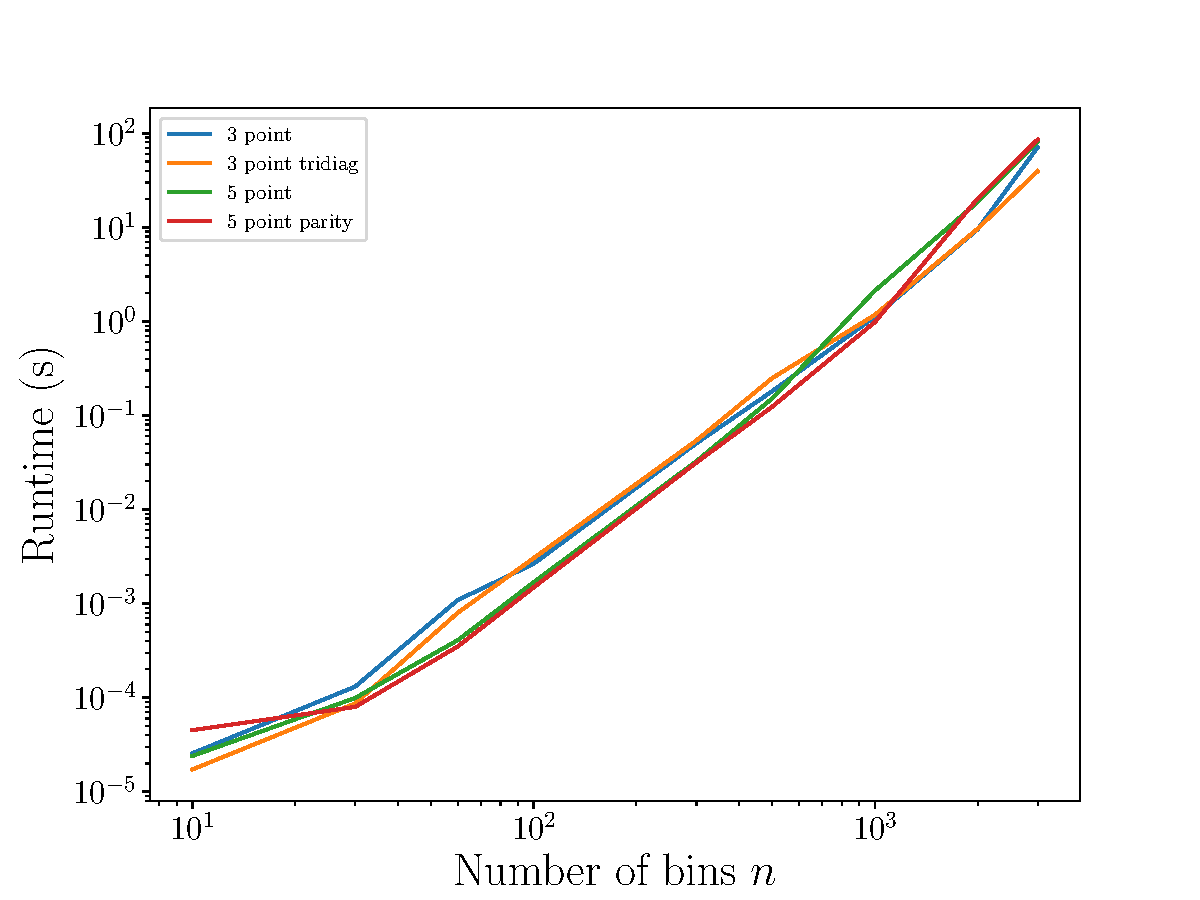
\includegraphics[width=0.65\textwidth]{../plots/bench/bench.pdf}
    \caption{Runtime of each solver plotted against the number of bins $n$. All are $O(n^3)$ and using parity brings a significant advantage for larger matrices. Inverse iteration performs best but was notably only used to find one eigenvector.}
    \label{fig:performance}
\end{figure}

The inverse iteration wins in this comparison, but it is to be noted that it was only used to find one eigenvector here. Since the $LU$-decomposition has to be calculated for every shift, the advantage this method has is quickly diminished when many eigenvectors are to be found. Also, if one does not have good guesses to their distribution, it can be difficult to avoid calculating the factorisation multiple times without finding a new eigenvector. This could be remedied by using full diagonalisation results for smaller matrices or estimating the distribution of the eigenvalues using, e.g., Gerschgorin circles which are numerically cheap.

\subsection{Discretisation Error}
There are two independent parameters that influence the trustworthiness of the eigenpairs: $n$ and $z_\text{max}$. To study their influence on the validity of the results, we first calculated the ground state energy of the harmonic oscillator for all the methods for various $n$, cf.~figure~\ref{subfig:bench_err_n}. Since we know the analytic result for the energies, we can examine the numerical error directly. It can clearly be seen that the error depends almost exclusively on the approximation of the derivative and not on the method. At some point, we would expect this to stop because the inverse iteration stops when the change in norm becomes less than $10^{-8}$. While the error falls of strongly with increasing $n$ for both formulae, the five-point formula yields better accuracy for smaller $n$ and should thus be preferred.
\begin{figure}
    \centering
    \begin{subfigure}{0.49\textwidth}
        \centering
        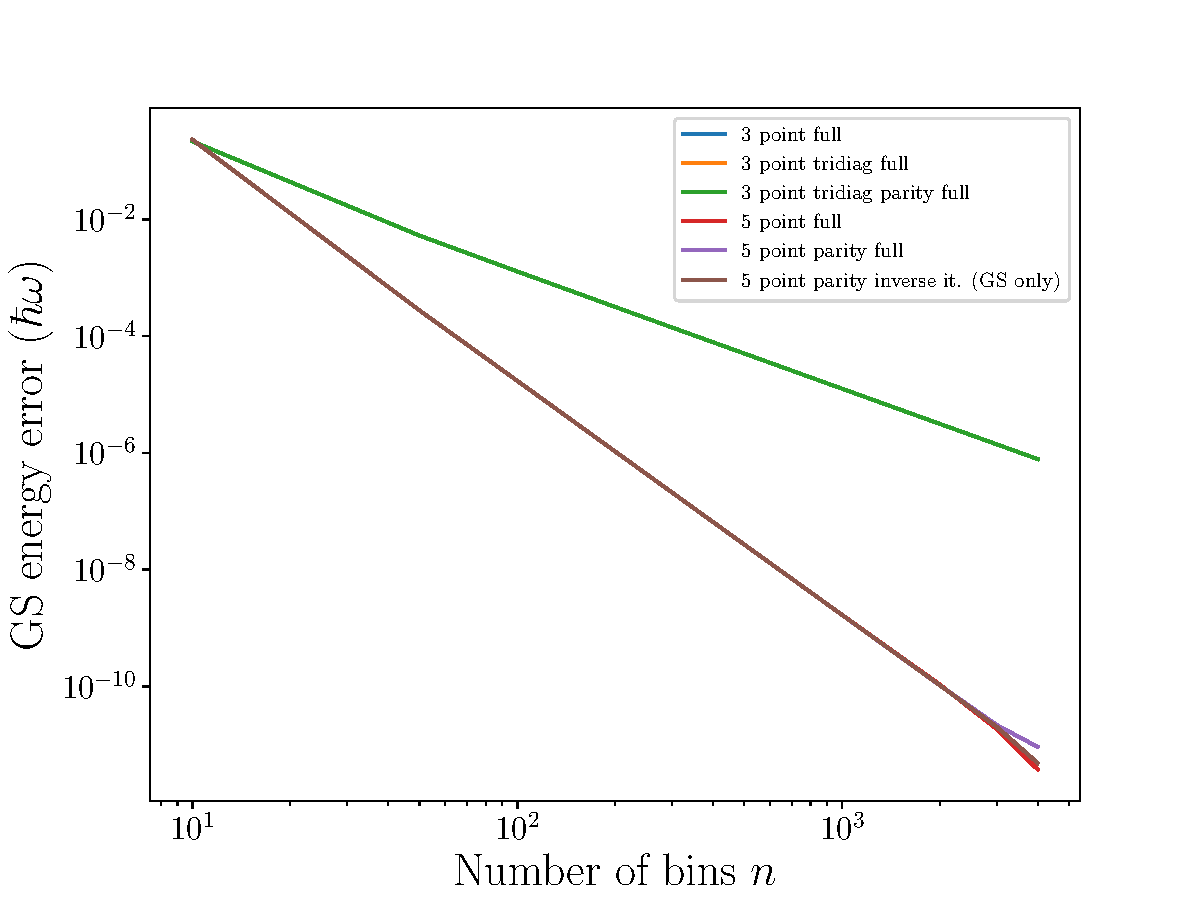
\includegraphics[width=\textwidth]{../plots/bench/bench_err.pdf}
        \caption{}
        \label{subfig:bench_err_n}
    \end{subfigure}
    \begin{subfigure}{0.49\textwidth}
        \centering
        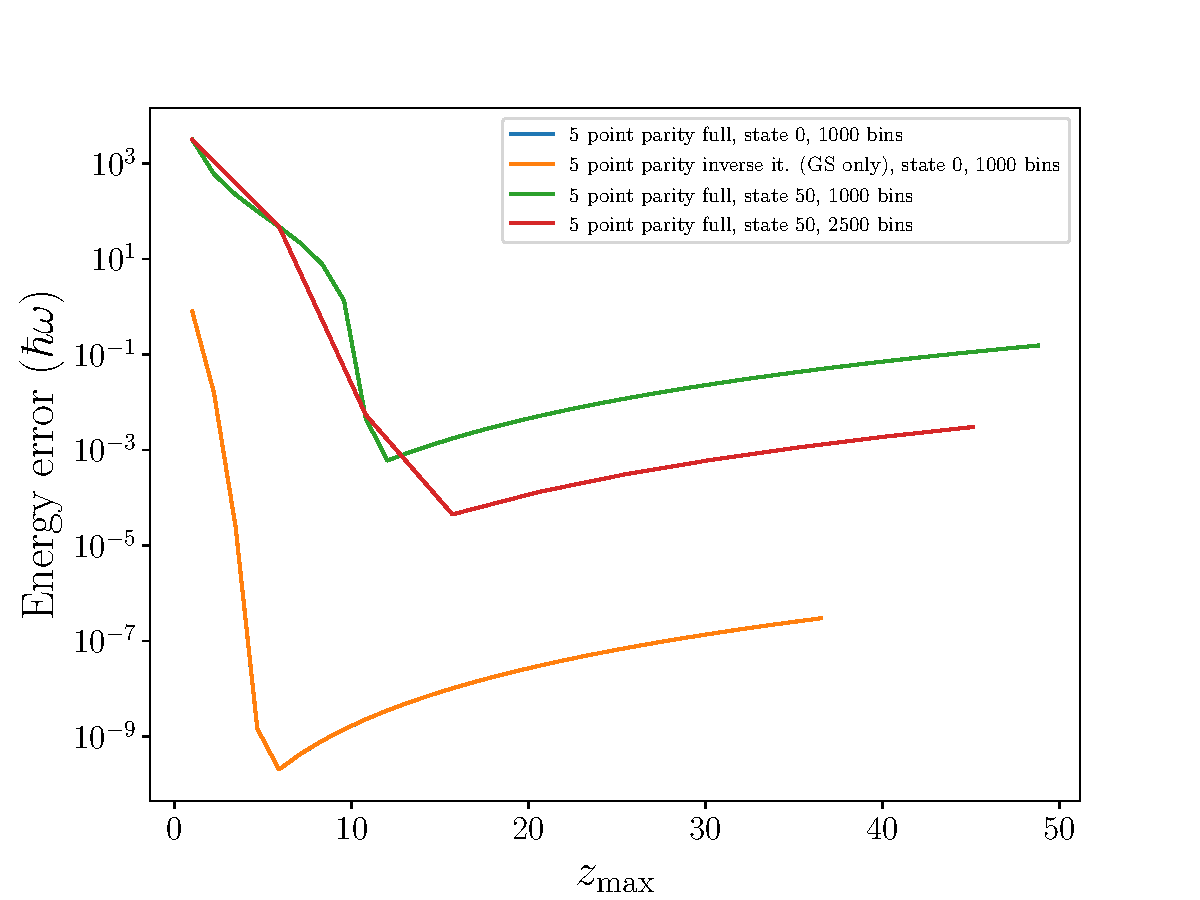
\includegraphics[width=\textwidth]{../plots/bench/bench_xmax_err.pdf}
        \caption{}
        \label{subfig:bench_err_zmax}
    \end{subfigure}
    \caption{Error of the numerically calculated energies for the ground state and varying $n$~\ref{subfig:bench_err_n} and for the ground and an excited state and varying $z_\text{max}$~\ref{subfig:bench_err_zmax}. The error depends almost exclusively on the approximation of the derivative and not on the method used and falls of strongly with increasing $n$. The five-point formula yields better accuracy for smaller $n$. For $z_\text{max}$, the behaviour of the error depends on the state in question.}
    \label{fig:bench_err}
\end{figure}

For $z_\text{max}$, the behaviour of the error depends strongly on the state in question. This is already true to an extent for varying $n$, but more so for $z_\text{max}$ because higher excited states are less localised around the minimum. For this reason, we show the error for the ground state and the 50th state for $n=1000, 2500$ in figure~\ref{subfig:bench_err_zmax}. As expected, a small box is sufficient to contain the maximally localised ground state while for an excited state, more space is needed. Informed by this, we chose to keep $z_\text{max}$ fixed at 20 henceforth to balance accuracy for the ground state and higher-lying states.

It is to be noted that while one can seemingly get quite a good approximation to the ground state energy with a small number of bins $n\approx 100$, this will not give a very smooth representation of the wave function which is localised on about $25\%$ of the interval $[-z_\text{max}, z_\text{max}]$, so even if the energies are already quite good, if one is interested in the states it might be prudent to go to higher $n$ regardless.

\subsection{Orthonormality}
Since $H$ is Hermitian, its eigenvectors should be orthogonal and can be chosen to be normalised (which we should require of physical states). We investigate this for $n=4000$ in figure~\ref{fig:orthonormal}, showing only the first $100$ states not because the observations do not hold for the rest but for visual clarity. We can see that the vectors are perfectly orthonormal within reasonable numeric accuracy ($\braket{i|j} < 10^{-18} \forall i\neq j$) as we should expect.
\begin{figure}
    \centering
    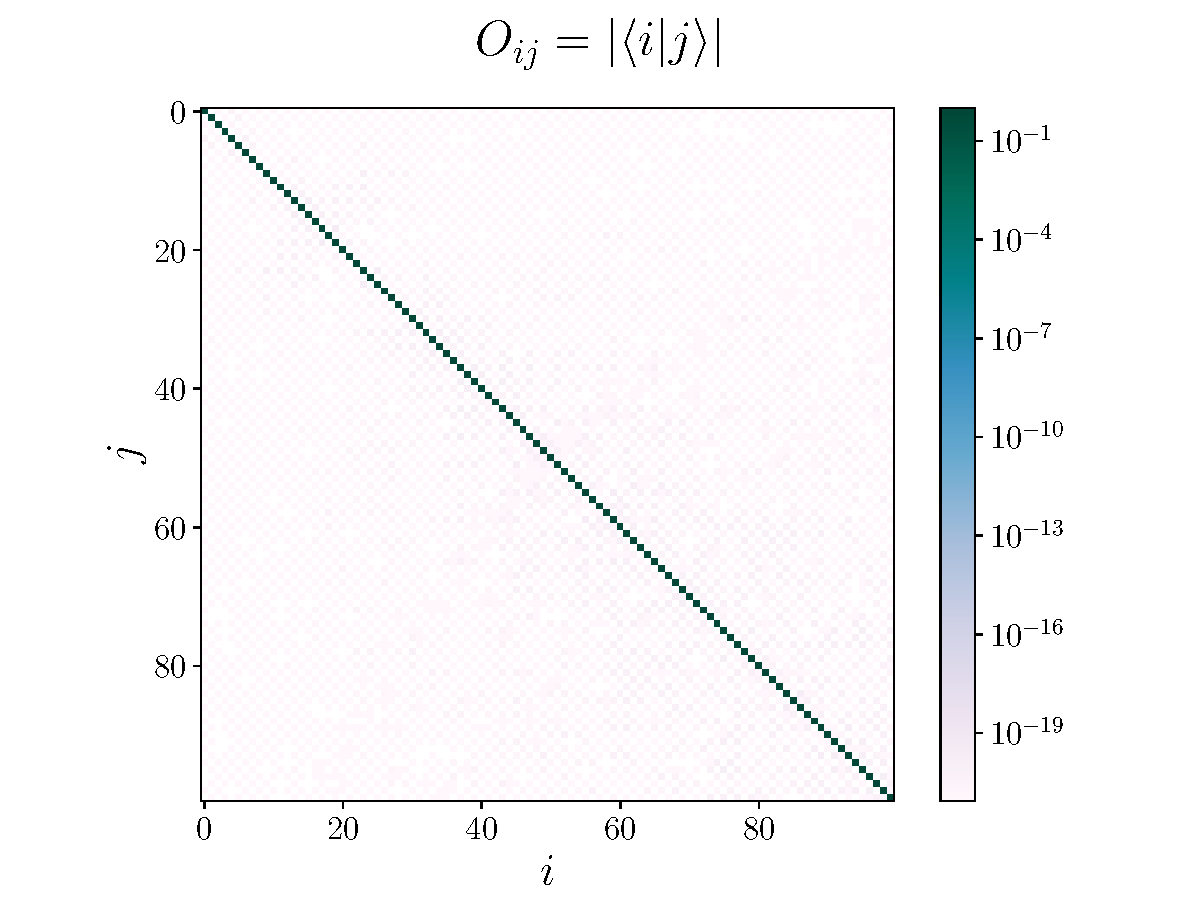
\includegraphics[width=0.65\textwidth]{../plots/orthonormal/orthonormality.pdf}
    \caption{Absolute value of the overlap of the first 100 eigenvectors for $n=4000$. The vectors are perfectly orthonormal as we should expect within reasonable numerical accuracy. }
    \label{fig:orthonormal}
\end{figure}

\FloatBarrier
\section{Results}
\subsection{Harmonic Oscillator}
\subsubsection{Eigenvalues}
We compare the numerical results of the eigenvalues obtained from full diagonalisation in figure~\ref{subfig:evals} and the deviation from the exact result in figure~\ref{subfig:evals_err}. It can be seen that around $i=200$, the energies begin diverging from the analytical result. In the errors, there appears a kink in the curve which might be exactly where this phenomenon begins. It is most likely due to the fact that such high lying states in the spectrum are highly spread out and begin not to \enquote{fit} into our box any more.
\begin{figure}
    \centering
    \begin{subfigure}{0.49\textwidth}
        \centering
        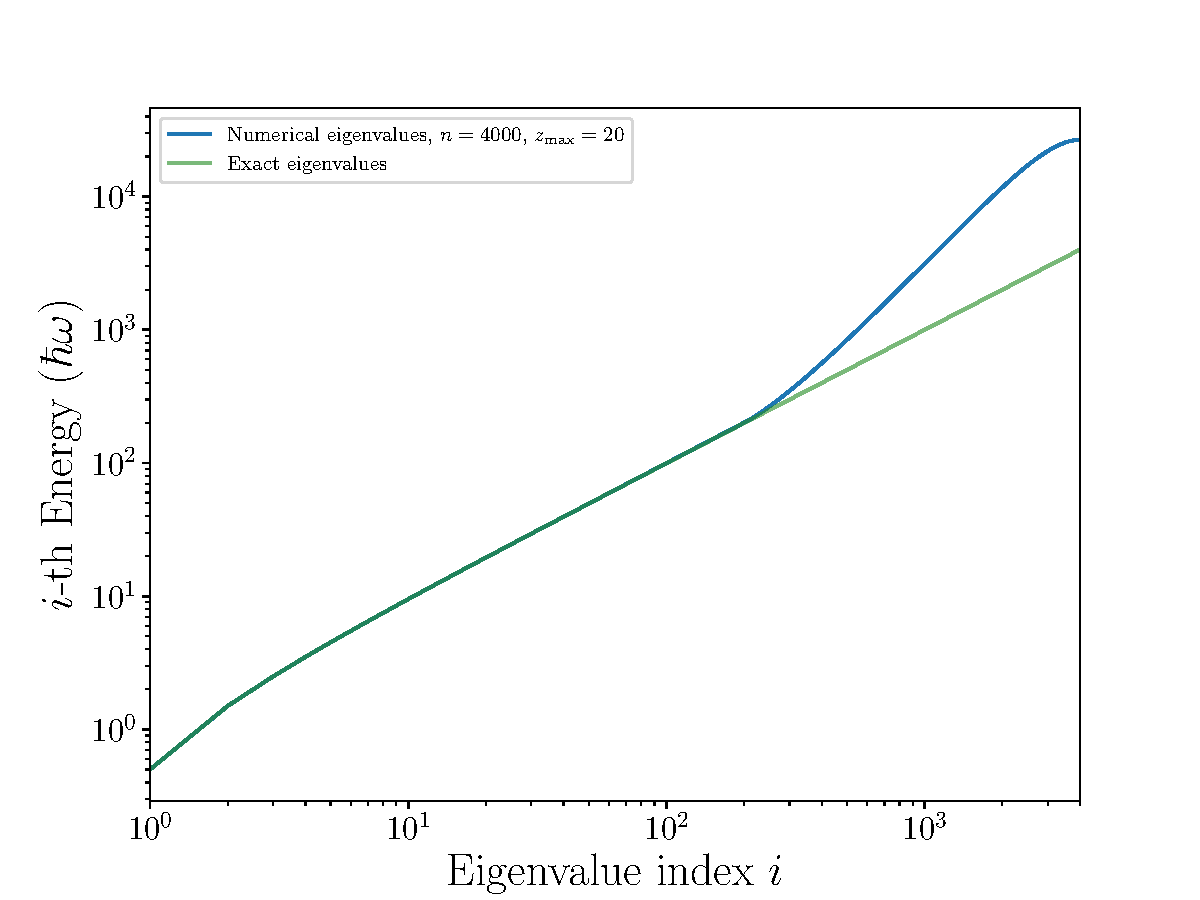
\includegraphics[width=\textwidth]{../plots/evals/evals.pdf}
        \caption{}
        \label{subfig:evals}
    \end{subfigure}
    \begin{subfigure}{0.49\textwidth}
        \centering
        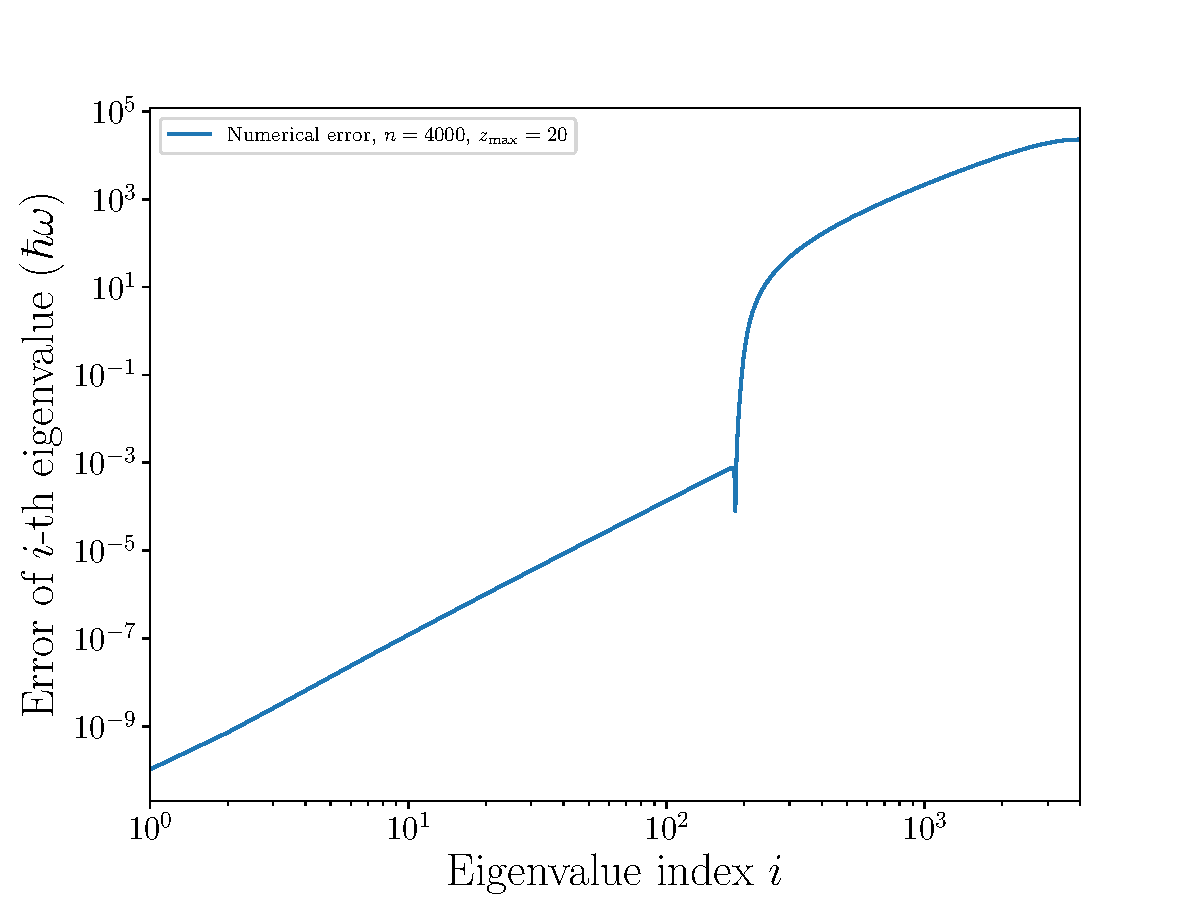
\includegraphics[width=\textwidth]{../plots/evals/evals_err.pdf}
        \caption{}
        \label{subfig:evals_err}
    \end{subfigure}
    \caption{Numerical eigenvalues for the harmonic potential with $n=4000$ and $z_\text{max}=20$. Around the 200th state, energies start majorly diverging from the analytic result.}
    \label{fig:evals}
\end{figure}

We omit a plot of the eigenvalues obtained using inverse iteration here because there is nothing else to be learned.

\subsubsection{States}
The first eight states obtained using full diagonalisation are shown in figure~\ref{fig:states}. We can see that they alternate in parity, obey the node theorem and become increasingly spread out with increasing energy. There was no time left to compare them to the analytic solution in a plot, but a rough visual comparison looks just fine.
\begin{figure}
    \centering
    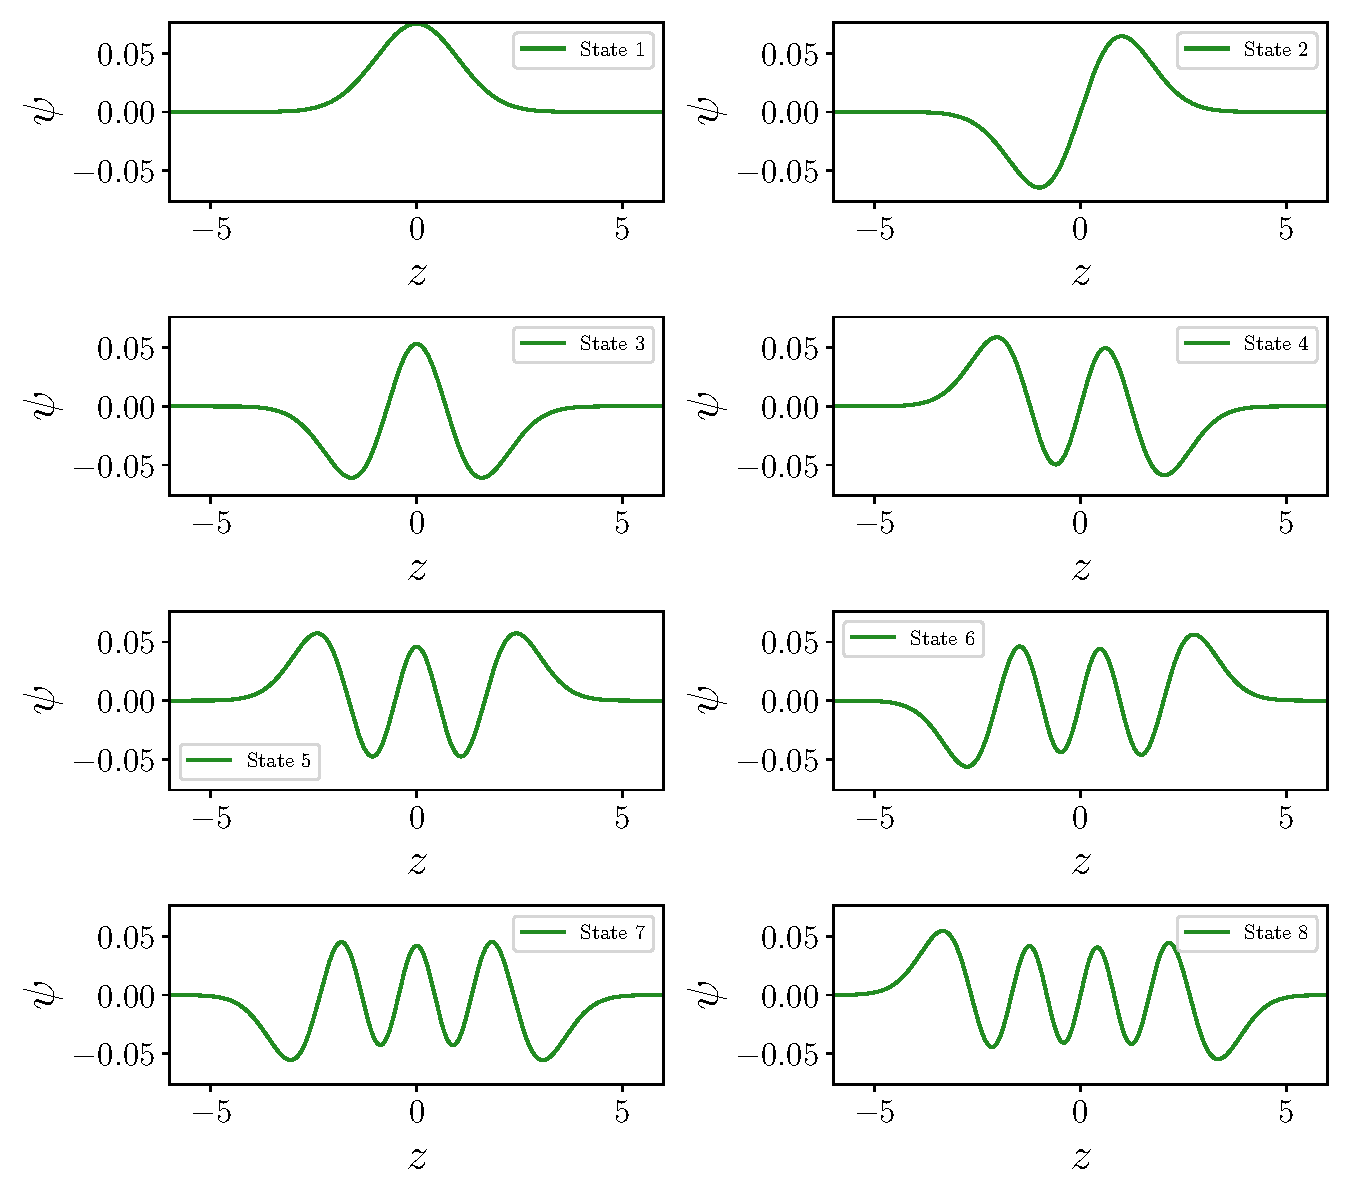
\includegraphics[width=0.8\textwidth]{../plots/states/states.pdf}
    \caption{First eight wave functions for the harmonic oscillator. They alternate in parity, obey the node theorem and become increasingly spread out with increasing energy as expected.}
    \label{fig:states}
\end{figure}
\begin{figure}
    \centering
    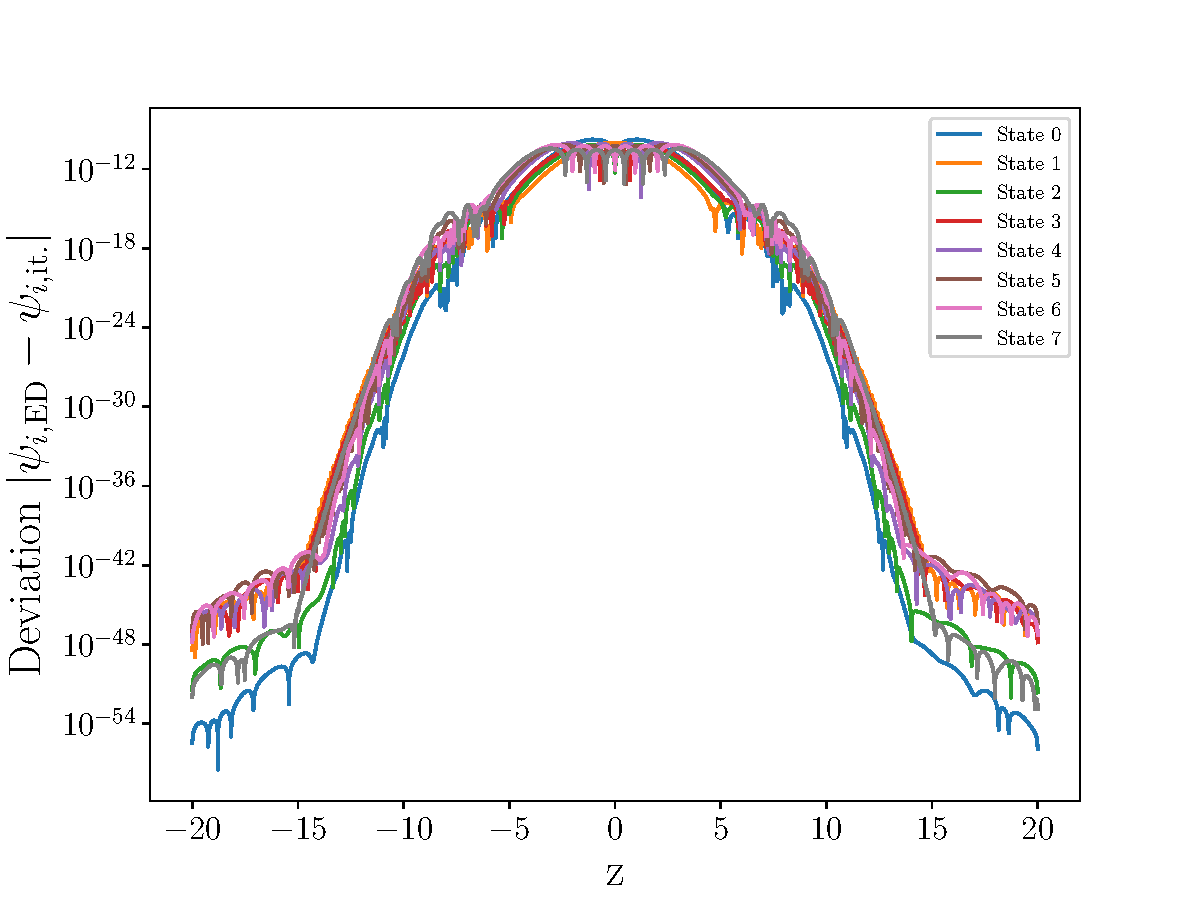
\includegraphics[width=0.65\textwidth]{../plots/states/deviation.pdf}
    \caption{Deviation between the first four full ED and inverse iteration states of the harmonic oscillator. The deviation is on the order of numerical error for all $z$.}
    \label{fig:states_invit}
\end{figure}

To judge the accuracy of the inverse iteration, we present the deviation between the first four full ED and inverse iteration states in figure~\ref{fig:states_invit}. We choose not to show the wave functions themselves again because there is no discernable difference to the naked eye. The errors show that agreement is very high.

High states found by our scheme are unphysical, see figure~\ref{fig:bad_states}.
\begin{figure}
    \centering
    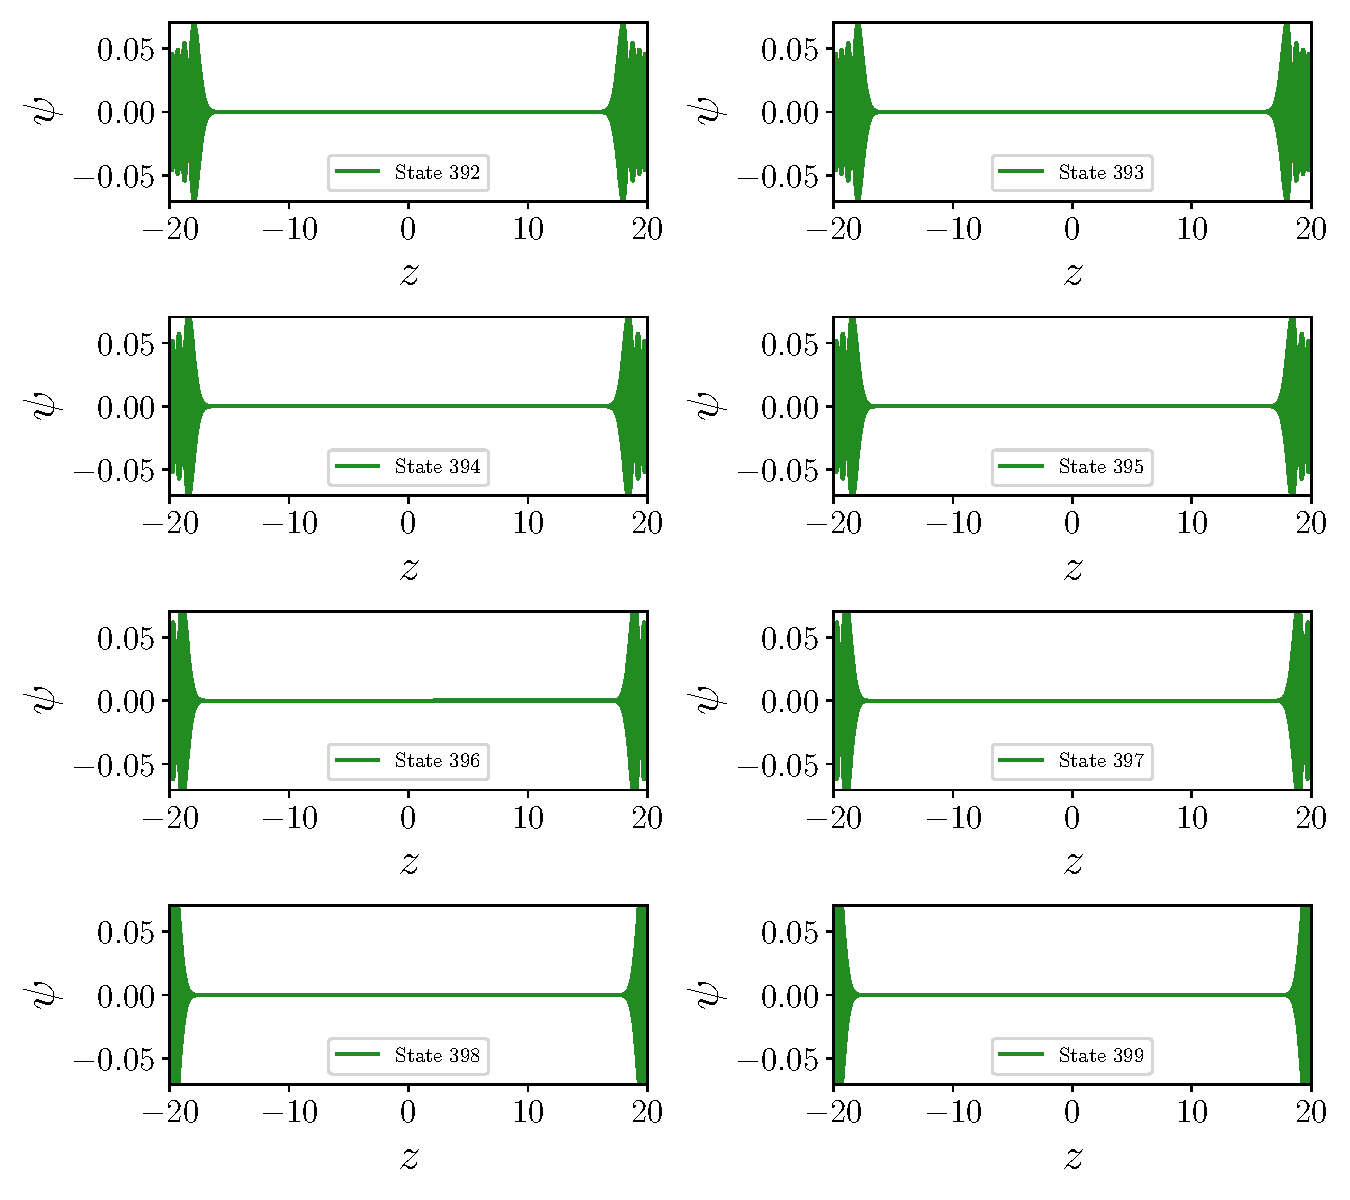
\includegraphics[width=0.8\textwidth]{../plots/states/states_high.pdf}
    \caption{Highest lying eigenstates found. These states are highly unphysical.}
    \label{fig:bad_states}
\end{figure}

Intermediate lying states near the point where the energies diverge from the correct result are still sufficiently physical to a coarse visual inspection, cf. figure~\ref{fig:ok_states}
\begin{figure}
    \centering
    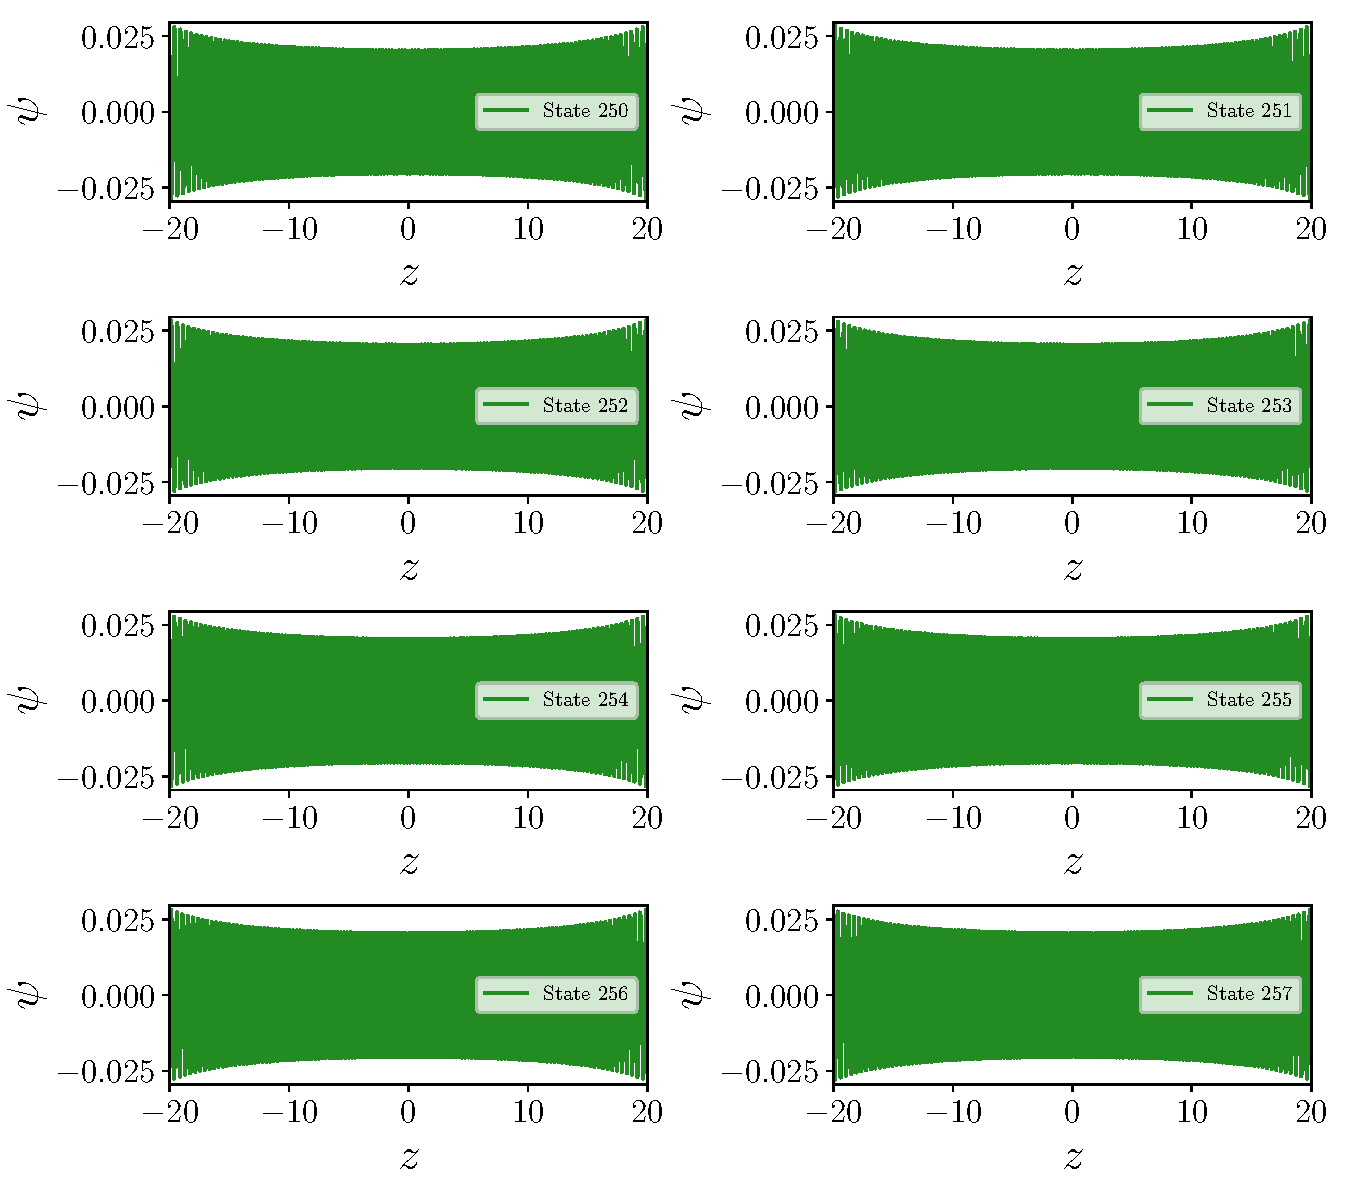
\includegraphics[width=0.8\textwidth]{../plots/states/states_low_middle.pdf}
    \caption{Intermediate eigenstates close to the point where they become unphysical. These states are not obviously unphysical yet.}
    \label{fig:ok_states}
\end{figure}

\subsubsection{Observables and algebra}
The physical states found all obey
\begin{equation}
    \braket{x} = 0, \quad \braket{p} = 0.
\end{equation}
The former is required of solutions to the SEQ for symmetric potentials. The latter is a general feature of bound states in quantum mechanics but also intuitively follows in this case from the fact that the wave function is real valued and $\mathcal{P}=-i\hbar\partial_x$. A rigorous proof uses partial integration and the fact that $\psi\in L_2$.

However, the expectation value $\braket{x^2}$ is non-zero and increases for higher lying states. According to Ehrenfest's theorem, for large $i$ this should approach the classical squared amplitude for a classical oscillator of the given energy, the two of which are proportional to each other. The numerically obtained expectation values are shown in figure~\ref{fig:pos2}. We observe the same behaviour as before, the values behave as expected until $i\approx 200$ when results become unphysical.
\begin{figure}
    \centering
    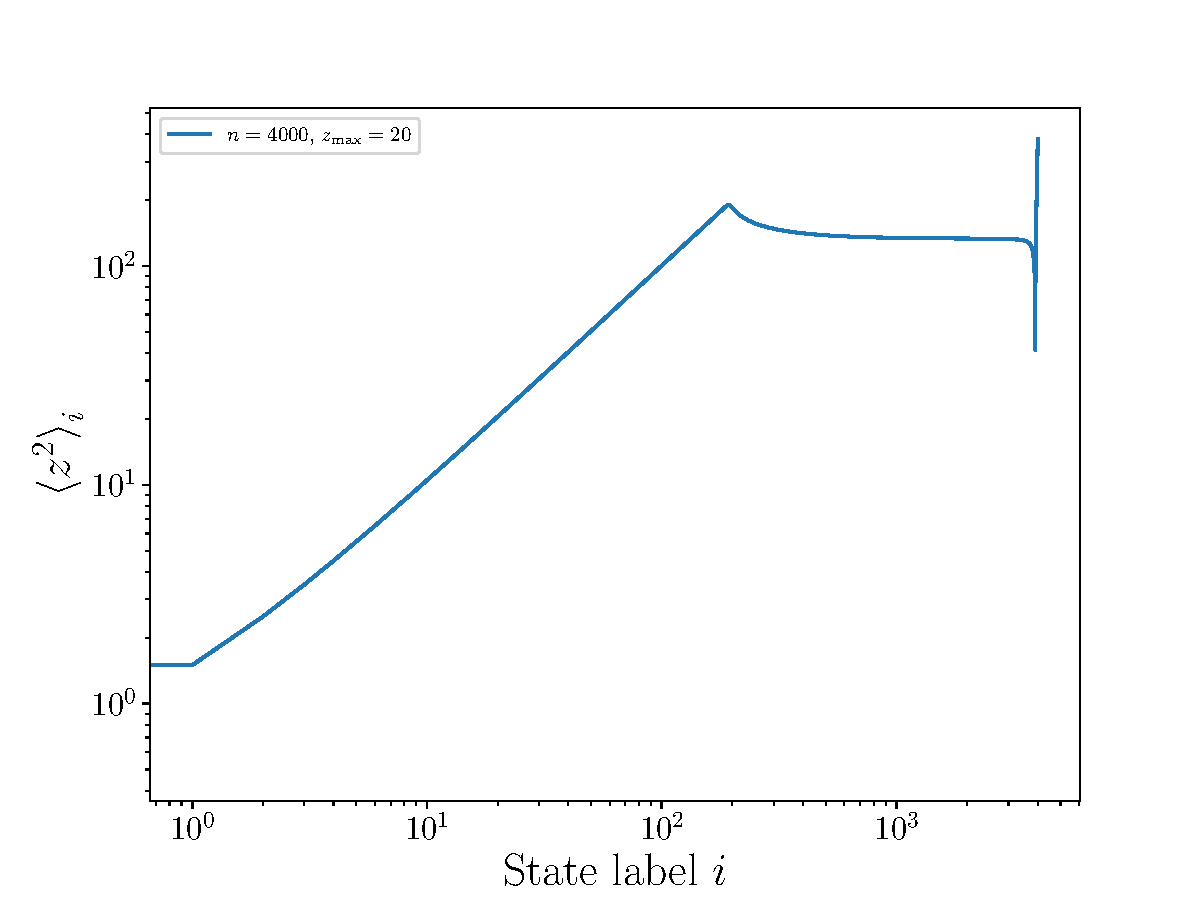
\includegraphics[width=0.65\textwidth]{../plots/pos2.pdf}
    \caption{Numerically obtained expectation values of the squared position operator.}
    \label{fig:pos2}
\end{figure}

The same can be seen with the expectation values of the number operator $n=a^\dag a$ shown in figure~\ref{fig:occupation}, where the ladder operators are given by
\begin{equation}
    a^\dag = \frac{1}{\sqrt{2}}\left(z - \partial_z\right)
\end{equation}
(recall that $\partial_z^\dag = -\partial_z$).
\begin{figure}
    \centering
    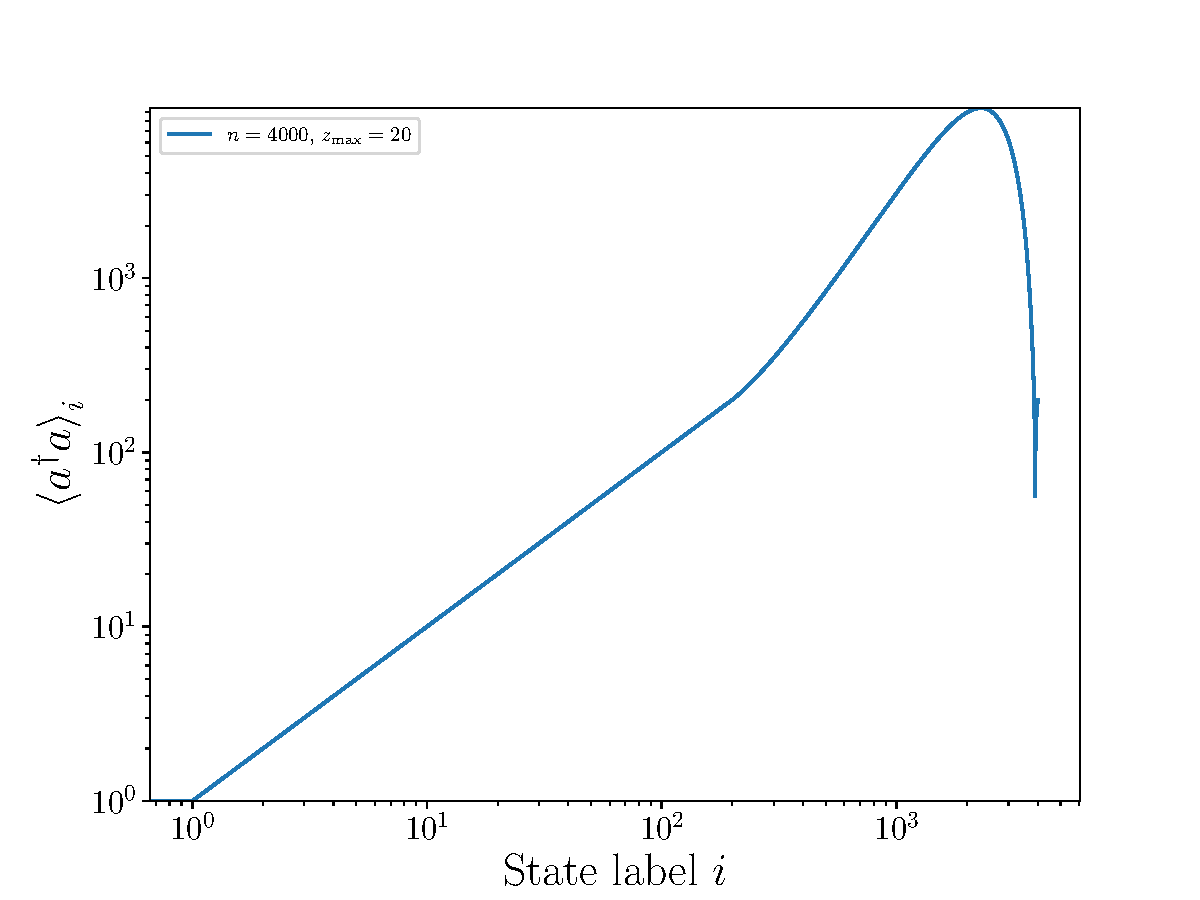
\includegraphics[width=0.65\textwidth]{../plots/occupation.pdf}
    \caption{Numerically obtained expectation values of the number operator.}
    \label{fig:occupation}
\end{figure}
Actually, an $\mathcal{H}$-eigenstate should also be an $n$-eigenstate since $\mathcal{H} = \hbar\omega\left(n + \frac{1}{2}\right)$.

As an aside, we were also able to transform the ground state into desired excited states using successive applications of the ladder operator, though this is somewhat outside the scope of this numerical analysis.

\FloatBarrier
\subsection{Modified Harmonic Oscillator}
We now want to consider a modified potential
\begin{equation}
    V'(z) = \frac{1}{2}z^2 + \alpha \text{e}^{-\beta z^2}.
\end{equation}
Note that this is also symmetric, so we can use parity states. We chose to study a small perturbation $(\alpha,\beta) = (1, 10)$ and a larger perturbation $(\alpha,\beta) = (5, 10)$, cf. figure~\ref{fig:pot}.
\begin{figure}
    \centering
    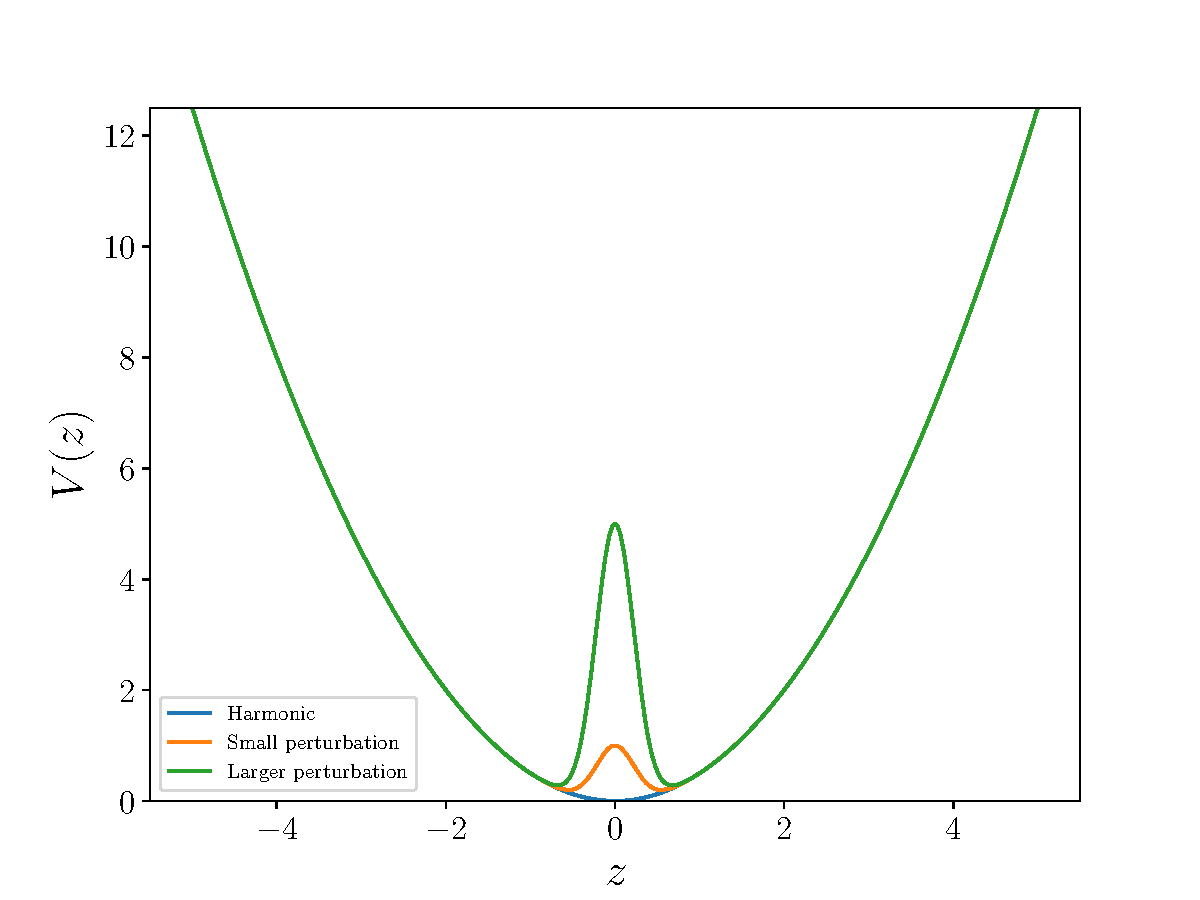
\includegraphics[width=0.65\textwidth]{../plots/pot.pdf}
    \caption{Unperturbed harmonic potential and perturbed potentials.}
    \label{fig:pot}
\end{figure}
\subsubsection{Eigenvalues}
Figure~\ref{fig:evals_bump} shows the deviation of the perturbed eigenvalues from the unperturbed oscillator for the first 100 states. We see that excited states are increasingly less affected by the perturbation, which makes sense because their probability densities are small near the perturbation and thus don't \enquote{feel} it as strongly. Additionally, the deviation is higher for even parity states, because they are more localised in the region of the perturbation.
\begin{figure}
    \centering
    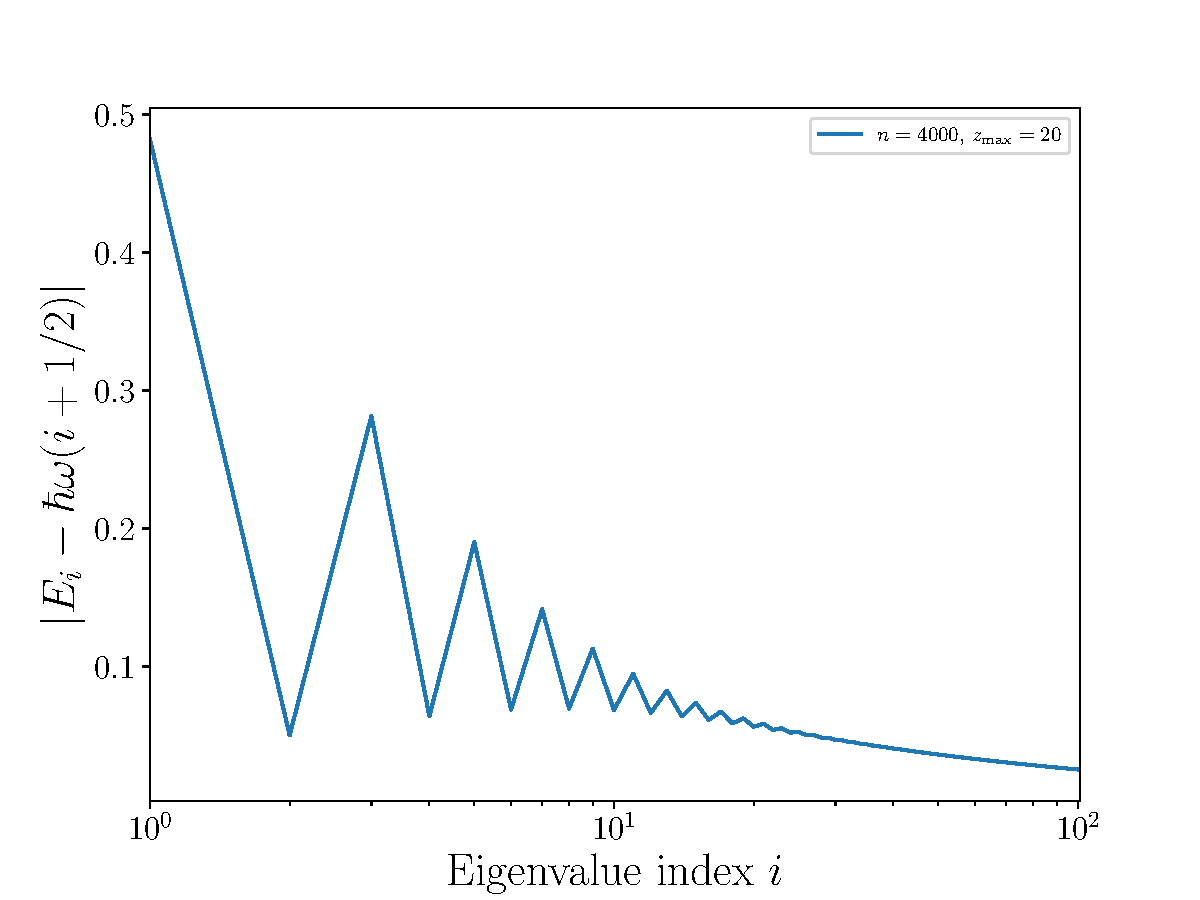
\includegraphics[width=0.65\textwidth]{../plots/evals/evals_bump.pdf}
    \caption{Deviation of the perturbed eigenvalues from the unperturbed oscillator for the first 100 states. Excited states are increasingly less affected by the perturbation, even states are more affected than odd ones.}
    \label{fig:evals_bump}
\end{figure}

\subsubsection{States}
The perturbed eigenstates of even parity show a clear deviation from the unperturbed states for small n, see figure~\ref{fig:states_comp}. However, for odd parity, even for the large perturbation the change in the wave function can barely be seen with the naked eye, which lines up with what we conjectured above.
\begin{figure}
    \centering
    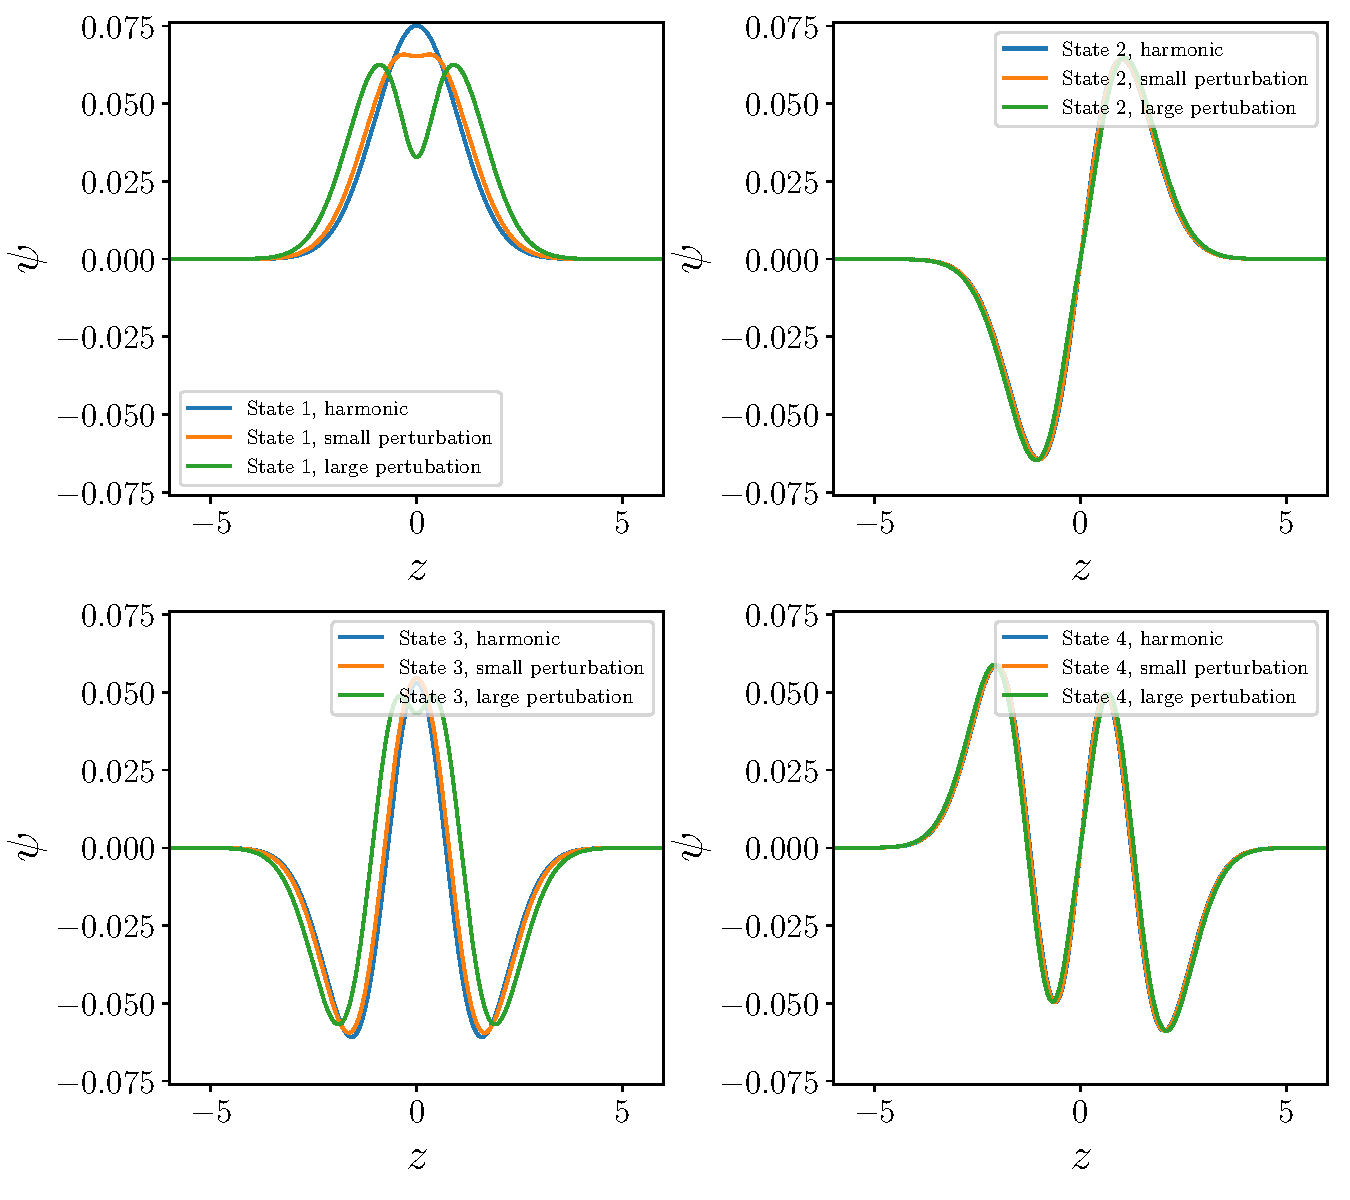
\includegraphics[width=0.8\textwidth]{../plots/states/states_comp.pdf}
    \caption{Comparison of the four first unperturbed and perturbed states. Odd states seem to be much less affected by the perturbation.}
    \label{fig:states_comp}
\end{figure}

\FloatBarrier
\section{Conclusion}
In this project, we successively implemented full diagonalisation and inverse iteration in a high level language. We applied the routines to the harmonic oscillator and verified our results by checking various general statements for symmetric potential and bound states and also  by comparing the energies to the exact solution.

Additionally, we investigated the effects of a slight perturbation in the potential on the states and energies.

\newpage
\FloatBarrier
\fakesection{References}
\printbibliography


\end{document}
